%====================================================
%====================================================
%====================================================
\newpage
\section{Décrire les objets audiovisuels (m)}\label{sec:desc}
\e{
Avant de commencer notre état de l'art sur la description des contenus audiovisuels, nous souhaitons préciser pourquoi et de quelle manière sont abordés la construction et la collecte de ces descriptions.
}
% Nous verrons quelles types de description chacune de ces approches construit sur les contenus, et comment ces descriptions sont exploitées, pour quel type d'usage, à l'intention de systèmes informatiques ou d'être humains.

\subsection{Quelles descriptions ?}
\paragraph{L'intérêt des descriptions textuelles}
Tout d'abord, nous souhaitons argumenter sur les avantages d'une description textuelle de contenus audio-visuels. 
En effet, pourquoi ne pas se contenter de ce que les images ont à nous offrir pour construire des index et rechercher ces images ? 
La question est d'autant plus pertinente que depuis presque une vingtaine d'années se développent des techniques évaluant la similarité entre images, ce qui permet d'utiliser une image (\gui{Query by Example}, initié par \cite{Flickner1995}, \cite{Pentland1996}) ou bien une représentation graphique (\gui{Query by Canvas}, initié par \cite{Flickner1995}, \cite{Bach1996}) comme élément de base pour une requête.
Ces approches sont donc tout à fait pertinentes dans le cadre de la recherche d'images extraites d'objets audiovisuels. 
Cependant, ces techniques reposent sur une caractérisation visuelle de l'image qui ne suffit pas à rendre compte de la richesse d'information que l'on voudrait associer aux objets audiovisuels.
En effet, de lui-même le contenu audiovisuel ne se laisse pas saisir dans son entièreté, ni ne se laisse manipuler aussi aisément que nous arrivons à le faire avec du texte. 
L'objet audiovisuel est avant tout temporel, il se déploie progressivement au fur et à mesure de sa lecture. 
On ne peut donc l'appréhender qu'en prenant le temps de le voir, instant après instant. 
À l'inverse, le texte est déployé dans l'espace ce qui lui permet d'être observé d'un point de vue synoptique. 
Ensuite, l'informatique manipule  bien plus aisément le texte que les contenus audiovisuels, surtout du point de vue de l'indexation. 
L'indexation textuelle utilise des mots-clés extraits directement du texte, mots-clés que l'on a appris à utiliser également pour effectuer une recherche d'information. 
De plus, les mots peuvent servir à décrire de multiple aspects de l'objet audiovisuel, qu'il s'agisse de nommer des éléments de l'image, de décrire sa composition, le contexte de sa production, son statut légal etc.
La limite d'une telle approche ne semble ainsi pas provenir du langage utilisé pour exprimer ces mots, mais plutôt de la manière de produire ces libellés. 
Nous écartons donc de notre état de l'art les recherches par images pour nous concentrer sur l'étude des modèles de description permettant de prendre en compte plusieurs aspects de l'objet audiovisuel. 


\paragraph{La diversité des descriptions}
La description d'un objet dépend fortement du point de vue de la personne qui la produit. 
En particulier, chaque corps de métier de la chaîne de production peut avoir une perspective particulière sur l'objet audiovisuel, même s'ils partagent des éléments communs pour discuter de sa production. 
Comme ces informations peuvent servir à de nombreux usages, il est intéressant de proposer des catégories permettant de les distinguer. 
Ainsi, \cite[\S 2:Types of Metadata]{Austerberry2004} distingue en particulier trois types d'informations : 
\begin{liste}
	\item \ciel{descriptive information} (informations descriptives) : qui sont relatives à la description du contenu, comme le sujet ou le genre de l'objet audiovisuel. 
	Par exemple, on peut associer des noms propres, des lieux, des évènements etc. à l'objet en fonction de ce dont traitera le contenu audiovisuel. 
	Un vocabulaire contrôlé peut servir à indiquer le "genre" de l'objet, c'est-à-dire les règles de genre qu'il suit au niveau de la structure, du ton etc.
	De même, des résumés textuels peuvent être inclus, à la manière de ceux prévus pour les guides TV. 

	\item \ciel{administrative information} (informations administratives) : qui relèvent de l'aspect métier et légal de la production de l'objet audiovisuel. 
	On cherchera à lister les contributeurs à la production de l'objet ainsi que les détenteurs de droits d'utilisation sur l'oeuvre. 
	Ces informations peuvent servir à retrouver des objets audiovisuels, notamment dans le cas de professionnels.
	Il peut également s'agir d'informations confidentielles comme les contrats de la distribution indiquant les droits d'utilisation de l'oeuvre, ou bien les contrats liées à la production. 
	Ces informations ne décrivent donc pas le contenu des objets audiovisuels, mais servent à faciliter leur gestion et leur exploitation future.

	\item \ciel{preservation information} (informations de conservation) : qui visent à faciliter la conservation et la réutilisation des objets et des fragments audiovisuels. 
	Il s'agit de pouvoir conserver des informations afin de faciliter la réutilisation de prises de vue dans de nouveaux contextes, de nouveaux montages ou bien de version spéciales suite à un changement de support de distribution. 
	De plus, cela peut aussi concerner le suivi des conditions de stockage des objets audiovisuels (lieux, support, état etc.) ou bien la réalisation d'opération de restauration. 
	Il s'agit donc d'informations qui permettent d'identifier et de pister non seulement les objets audiovisuels finis, mais également tous les fragments qui ont été crées à l'occasion et toutes les versions qui ont été construites par la suite.
\end{liste}


Nous pouvons ajouter à ces catégories, d'autres types d'informations proposées par \cite{Rayers2002} : 
\begin{liste} 
	\item \ciel{compositional information} (informations de composition) : qui identifient la liste des fragments composant un objet audiovisuel et la manière dont ils doivent être montés pour reconstruire l'objet. 
	Dans le milieu de l'audiovisuel, ces informations sont représentés sous la forme de ce qu'on appelle une \ciel{Edit Decision List} (EDL).
	Cette liste peut être produite soit sous forme papier, soit par un logiciel de montage en utilisant une des dizaines de formats existants, formats souvent propriétaires et liés au logiciel de montage. 
	Ces informations servent à décrire la structure des objets audiovisuels et peuvent servir à leur gestion.
	Elles sont à rapprocher des \ciel{preservation information} dans le sens où elles permettent de garder trace du montage. 


	\item \ciel{technical or essential information} (informations techniques) : qui correspondent à une description techniques des caractéristiques du signal audio-visuel. 
	Ces informations sont généralement présentes dans les formats d'encapsulation de contenu numérique afin de permettre son décodage.
	Ces informations peuvent également servir à différencier plusieurs versions d'un objet audiovisuel qui ne varieraient que par leur encodage. 
	Il s'agirait alors de rapprocher ces versions avec leur utilisation futures (utilisation comme proxy, version destiné à un support particulier, à un canal de distribution etc.).
\end{liste}


Notons enfin, qu'il existe également toutes sortes de descriptions produites par des intervenants extérieurs à la chaîne de production (les spectateurs, les critiques, les sémiologues etc.).
% pertinent pour notre problème.



\subsection{Comment construire les descriptions ?} 
\subsubsection{La collecte durant la production}
Dans la chaîne de production audiovisuelle, chaque communauté de contributeurs a un intérêt particulier et souvent différent sur les informations à partager sur l'objet. 
Les informations que l'un jugera critique (sur quelle cassettes peut-on trouver la prise de vue n°354) peuvent être jugé insignifiante pour d'autres (un journaliste se contentera de savoir que la prise de vue existe). 
Il existe donc autant de descriptions possible d'un objet, que de point de vue sur cet objet. 
De plus, une description n'est jamais utile qu'en fonction d'un usage. 
Savoir où se trouve la prise de vue n'a d'intérêt que pour la personne qui devra en réaliser le montage, ou bien s'assurer de la préservation de la cassette une fois utilisé. 
Les professionnels de la production sont donc confrontés à de multiples informations, pas forcément pertinentes par rapport à la tâche qu'ils doivent réaliser mais qui peuvent s'avérer utile plus loin dans la chaîne.  

\citeauthor{Rayers2002} et \cite{Austerberry2004} présentent en détails la manière dont les informations sont produites dans les processus de production télévisuels. 
Leur expertise\footnote{Ces auteurs ont travaillé, entre autres, pour les réseaux de télévision public anglais (BBC), néerlandais (NOS), une bouquet privé américain (HBO) et en collaboration avec la principale association de professionnels du milieu de la télévision (SMPTE).} indique que ces informations
sont collectées, manipulées,  réutilisées, diffusées à différentes étapes de la chaîne de production. 
Pourtant, la mise en commun de ces informations restent un défi et il semble fréquent que ces informations doivent être retrouvés à la main, voire reconstruite à défaut d'en avoir connaissance :

\ciel{
	However, the point in the process where a piece of metadata first becomes available is not necessarily a point where it is needed for that stage in the process. Worse, frequently two or more stages in the workflow might need the same metadata, but not the intervening processes.} (\cite[p.22, Metadata in the Workflow]{Austerberry2004})

De même, il semble également que la structuration de ces informations se fassent le plus tard possible, c'est-à-dire au moment de l'archivage, à partir des mêmes informations utilisés pour construire les programmes TV\footnote{En plus, des citations que nous avons trouvé dans des livres d'experts, nos partenaires du milieu de l'audiovisuel dans le projet MediaMap nous ont également confirmé ce problème. Il s'agissait d'ailleurs d'un des problèmes centraux auquel le projet MediaMap s'est attaqué.}.
L'accès aux informations constituées pendant le déroulement de la chaîne est donc très difficile une fois la production finie.
Ainsi, les auteurs proposent de favoriser une collecte des informations au fur et à mesure de la chaîne afin d'éviter toute perte de temps mais aussi de favoriser le partage et la qualité des informations : 

\ciel{
	Clearly, it makes sens to capture metadata at the earliest stage possible as a program is made, and to either pass it through the chain or hold it in a common repository. This way, those stages that need the metadata can access it easily and do not need to look for it, reacquire it, or, worse, reinvent it. Sadly, this has \e{not} been the traditional way of doing things.} (\cite[p.23, Metadata in the Workflow]{Austerberry2004})

\ciel{
	At each step in the production process we can collect, and possibly re-use metadata. [\dots] Each re-use point is a saving as we have removed a data re- entry, probably reduced errors and given producers more information to help their task.} (\cite{Rayers2002})

% collecte de MD tout au long de la chaîne : \cite{Rayers2002}



\subsubsection{La construction a posteriori}
Les approches classiques de construction de descriptions des contenus audiovisuels se font \e{a posteriori} de la production de l'objet audiovisuel. 
Elles interviennent en fin de chaîne, après la diffusion, voire en-dehors lorsqu'un organisme différent du producteur se charge de l'archivage (c'est le cas de l'INA avec l'audiovisuel public en France). 
Il faut distinguer deux genres d'approches pour construire des descriptions de contenus audiovisuels : 
\begin{liste}
	\item les approches automatisées qui procédent par analyse du signal audio-visuel pour décrire le contenu.
	Par exemple, un programme qui réalise une transcription des paroles prononcés dans une émission, ou bien un système de détection de changement de plans. 

	\item les approches manuelles où un humain, éventuellement assisté par un système informatique, produit une interprétation du contenu avant de le décrire. 
	Il peut s'agir par exemple d'un documentaliste qui classifie et résume le contenu d'une émission dans un système d'archivage.
\end{liste}

\paragraph{L'analyse automatique du signal}
\cite{Staab2008} propose d'examiner les nombreux travaux menés suivant l'approche automatisée. 
De manière générale, ces travaux analyse le signal audio-vidéo pour en extraire par calcul un ensemble de composantes (feature).
Par exemple, le signal vidéo peut être décomposé en termes de couleur, de texture, de forme, de mouvement etc. 
Ces composantes servent ensuite de données d'entrée à des classifieurs qui cherchent à identifier des objets pour en fournir un libellé. 
De multiple sortes d'analyses peuvent être menées automatiquement à partir du signal ou bien de documents annexes comme le rapportent \cite[\S 8 : Cataloguing and indexing]{Austerberry2004} : 
\begin{liste}
	\item \e{analyse de texte} : lorsque des éléments textuels sont fournis avec le matériel audiovisuel, il est alors possible de les analyser pour en extraire des métadonnées. 
	Il peut s'agir par exemple d'un fichier de sous-titre, d'une retranscription textuelle destiné aux malentendants, d'un résumé du programme etc. 
	Mais cela pourrait également s'appliquer directement à des documents de production.

	\item \e{analyse audio} : la première distinction que l'on cherche à effectuer est de savoir si la séquence étudiée contient de la musique, un discours ou bien simplement s'il s'agit de silence.
	Lorsqu'il y a discours ou dialogue, on peut ensuite tenter de faire de la reconnaissance de paroles (pour obtenur une retranscription) et une reconnaissance des intervenants (combien de personnes parlent dans cette séquence, qui dit quoi ?) voire une identification des orateurs à partir de leur voix. 
	Pour la musique, on pourrait chercher de même à identifier l'interprétation et récuperer les métadonnées correspondantes. 

	\item \e{analyse vidéo} : l'analyse vidéo vise principalement à reconnaître des objets, des visages ou des éléments de textes dans les images. 
	La reconnaissance de visages permet d'identifier le nombre de personnes présentes à l'image voire de les identifier à partir d'une base de données. 
	La reconnaissance de caractères permet par exemple de produire une retranscription des titres d'un journal télévisé ou tout autre texte à l'écran juste avec le signal vidéo. 
	De nombreuses autres types d'analyses peuvent être menées, la reconnaissance d'objets ou bien encore la détection des mouvements de caméra. 
\end{liste}


% description humaines (sémiotique des contenus par exemple)


\paragraph{À propos du fossé sémantique}
% décrire le signal par des descripteurs analytiques/objectifs
Comme nous avons vu, les approches d'analyse du signal audio ou vidéo visent donc à reconnaître puis à nommer ou identifier un certain types d'objets présent dans un objet audiovisuel. 
Cependant, \cite{hare:semantic-gap} pointe la limite de la description par libellé qui ne propose pas d'interprétation aussi complète que celle effectuée par un humain. 
Il propose l'exemple d'une image montrant une manifestation où l'on voit des étudiants et des policiers. 
Si l'analyse permettra d'indiquer le nombre de gens, de reconnaître des bâtiments ou des véhicules, voire le mot police, le fait de nommer ces éléments ne permet pas de conclure qu'il s'agit d'une manifestation. 
Cet écart entre les résultats de l'analyse automatique du signal et l'interprétation humaine se nomme ainsi le \gui{fossé sémantique} (semantic gap). 


\citeauthor{hare:semantic-gap} caractérise alors ce fossé en deux sous-problèmes distincts : 

\ciel{
It may be instructive to see the gap in two major sections, the gap between the descriptors and object labels and the gap between the labelled objects and the full semantics.}

En d'autres termes, reconnaître et nommer à partir du signal n'est que la première difficulté à surmonter, il s'agit là d'un problème d'ordre calculatoire qui fait l'objet d'un très grand nombre de travaux.
Le second problème consiste à passer d'une description par libellés à une description proche de l'interprétation humaine, ou tout du moins un certain type d'interprétation humaine. 
On retrouve cette caractérisation du fossé sémantique en deux étapes différenciés dans la définition proposé par \cite{Smeulders2000} et reprise dans l'\e{Encyclopedia of Multimedia} (\cite{Furht2008}) :  %!!ref

\ciel{
	The semantic gap is due to two inherent problems. 
	One problem is that the extraction of complete semantics from image data is extremely hard as it demands general object recognition and understanding. [\dots]
	The other problem causing the semantic gap is the complexity, ambiguity and subjectivity in user interpretation.}

Si les libellés ne suffisent pas à décrire les objets audiovisuels pour des agents humains, \citeauthor{hare:semantic-gap} propose de s'intéresser aux besoins de ces agents et notamment aux requêtes qu'ils souhaitent poser et aux raisonnements que le système d'indexation doit pouvoir effectuer. 
L'exemple pris est celui d'une requête d'une photo d'un frigo des années 50. 
Dans ce cas, la requête mentionne un nom de marque qui ne correspond pas au nom commun pour ce type d'appareil (réfrigérateur). 
Ainsi, l'attente implicite serait de pouvoir effectuer des rapprochements sémantiques entre libellés de la requête et libellés utilisé dans l'indexation. 
Ce qui suppose l'utilisation de vocabulaire structuré à la base de l'indexation et un formalisme permettant d'effectuer des raisonnements. 

\e{
Dans notre cas, nous nous intéressons à la manière dont les utilisateurs recherchent des séquences vidéos dans les pratiques de réutilisation des objets audiovisuels (décrites précédemment en section \ref{sec:reuse}). 
Or, il s'agit maintenant d'examiner les moyens de décrire ces objets audiovisuels en regard de ces pratiques de réutilisation. 
Ainsi, nous nous attacherons dans cette section à présenter les standards, modèles et vocabulaires qui contribuent à décrire les objets audiovisuels. 
Nous détaillerons quelles sont les informations fournies par ces modèles et quel genre de manipulation des objets audiovisuels elles permettent d'effectuer.}




%=============================
%=============================
% \subsection{Modèles et standards de description}
% News-ML (\cite{Nack2004}) etc.

% \begin{figure}[ht!]
% \centering
% 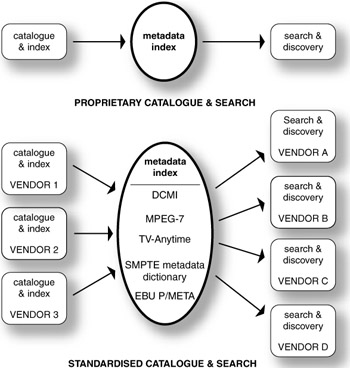
\includegraphics[width=0.6\textwidth]{images/standards-description.jpg}
% \caption{Une vision  de l'indexation et une recherche interopérable utilisant les  principaux standards }
% \label{img:soa:standards}
% \end{figure}




%=============
\subsection{MPEG-7 Part 5: Multimedia Description Scheme}
% \cite{Hunter2001} ; \cite{Troncy2007} ; \cite{Nack2005a} ; \cite{Dasiopoulou2009} ; \cite{Garcia2005} ; 

% à revoir
Parmi les normes utilisés pour décrire le contenu des audiovisuels, MPEG-7 est certainement devenu le standard de l'industrie. 
Développé à partir de 1998 par le comité MPEG (Moving Picture Expert Group) à la suite des standards MPEG-1, MPEG-2 (norme de compression du signal audiovisuel) et MPEG-4 (norme de d'encodage multimédia basée sur les objets), MPEG-7 est devenu une norme ISO/IEC en 2001 puis mise à jour jusqu'en 2006. 

La norme définit un ensemble de \e{Descripteurs} (Descriptors, Ds) dont les valeurs permettent de caractériser un objet audiovisuel, qu'il s'agisse de composantes du signal ou bien d'autres aspects comme des informations relatives à sa création, sa structure, son usage passé et futurs etc.
Ces Descripteurs sont organisés en \e{Schémas de Descriptions} (Description Schemas, DSs) dont on peut avoir une vue d'ensemble dans la Figure \ref{img:soa:mds}.
C'est cette partie de la norme (\cite[Part 5 : Multimedia Description Scheme]{ISO/IEC2004}) que nous traiterons en particulier dans cette section. 

\begin{figure}[ht!]
\centering
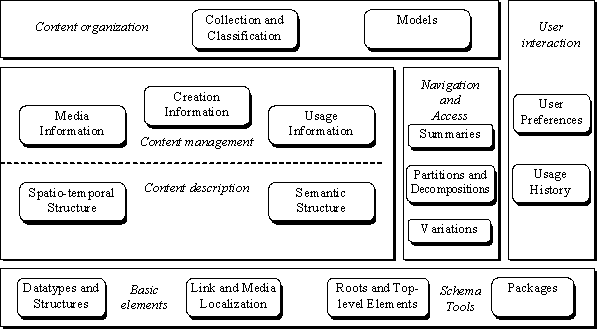
\includegraphics[width=0.8\textwidth]{images/MPEG-7-MDS.png}
\caption{Vue d'ensemble des Schémas de Description (DSs) de la norme MPEG-7}
\label{img:soa:mds}
\end{figure}

Les descriptions produites sont représentées dans un \e{Langage de Description des Définitions} (Description Definition Language, DLL) qui permet de spécifier la syntaxe des Descripteurs, la structure des Schémas de Description ainsi que la sémantique de l'ensemble.
Ce langage permet également de créer ou modifier des Descripteurs, d'étendre ou de modifier les Schémas de Descriptions. 
Le DLL est en réalité XML Schema (\cite{Fallside2004}) agrémenté de quelques types primitifs.

Pour utiliser MPEG-7, il faut également des outils et des directives annexes qui permettent de guider les utilisateurs. 
% définition / implémentation ? 
Dans la partie \e{Systems} de la norme, on trouve ainsi la définition d'outils qui remplissent les fonctions suivantes : codage d'une description MPEG-7 en binaire ; mécanismes de transmissions des descriptions (en binaire ou en texte) à part ou en parallèle du contenu audiovisuel décrit ;  synchronisation entre description et contenu audiovisuel ; gestion des descriptions et de la propriété intellectuelle. 
La partie \e{Reference Software} présente des logiciels de références pour utiliser la norme.
Enfin, la partie \e{Conformance} explicite des directives et des procédures pour s'assurer de la conformité des descriptions produites.

Nous détaillerons dans cette section les Schémas de Description liés à la gestion du contenu (\e{Content Management} dans la Figure \ref{img:soa:mds}) et à la description du contenu (\e{Content Description}).\\


\subsubsection{Gestion du contenu}
MPEG-7 définit trois concepts fondamentaux pour modéliser l'enregistrement d'une réalité en un contenu multimédia et les multiples transformations qu'il est possible de lui appliquer. 
Ainsi, pour chaque modalité d'enregistrement (audio, audiovisuel, photo etc.) MPEG-7 considère la création de trois éléments, une \pc{Content Entity} (entité de contenu, CE), une \pc{MediaInstance} (instance de média, MI) et un \pc{MediaProfile} (profil de média, MP), voir la Figure \ref{img:soa:media}.
Pour donner une première idée, on peut dire que le fichier créé correspond à la \pc{MediaInstance}, que le \pc{MediaProfile} correspond aux paramétrages de son encodage et que la \pc{Content Entity} représente le contenu de manière abstraite.

\begin{figure}[ht!]
\centering
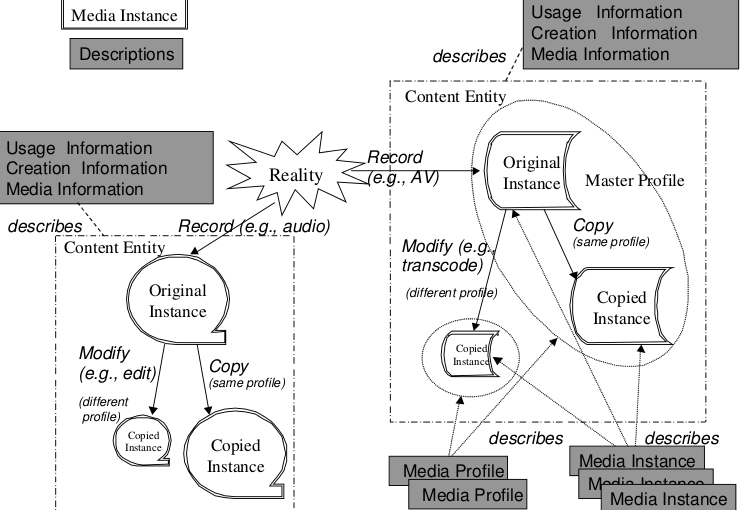
\includegraphics[width=0.8\textwidth]{images/MPEG-7-MediaManagement.png}
\caption{Gestion des contenus dans MPEG-7 à trois niveaux : contenu, instance et profile (extrait de la norme).}
\label{img:soa:media}
\end{figure}


On remarque qu'il existe cependant des différences entre les \pc{MediaInstance}, entre l'original et ce qui est nommé des \gui{copies} (copied instances). 
Ce qui est particulièrement intéressant pour nous est de constater que la nature de la manipulation entre l'original et les soi-disantes \gui{copies} importe peu (copie technique, réencodage ou montage), car cela crée de toute façon une nouvelle \pc{MediaInstance}. 

À l'inverse, la notion de \pc{MediaProfile} est dépendante de la nature de ces transformations. 
Le \gui{MasterProfile} correspond ainsi aux paramètres d'encodage de la MI d'origine, la première créée. 
Ainsi, dès qu'une différence d'encodage apparaît avec les MI créées ultérieurement, un nouveau \pc{MediaProfile} est créé. 
Il correspond donc à un regroupement de toutes les instances ayant en commun le même encodage. 
%%%% orthographe %%%%
Ce qui paraît troublant néanmoins, est l'amalgame fait entre réencodage et montage. 
Les changements de structure réalisés par le montage semblent en effet bien plus significatif qu'un changement de paramètre d'enregistrement. 
On peut se souvenir de la citation d'\pc{Eisenstein} à ce sujet évoqué en section \ref{sec:prod}.

Enfin, la notion de \pc{Content Entity} correspond à une entité abstraite permettant de regrouper toutes les versions ultérieures de ce même contenu.
De ce fait, c'est à elle qu'on attache des informations concernant la création, l'usage et le type de média construit. % ??? Sûr ???
Ce regroupement d'informations à ce niveau découle de l'idée que chaque \pc{Content Entity} définit une forme reconnaissable de contenu, quelque soit les variations apportées.
Encore une fois, l'idée qu'un montage différent n'impacte pas la forme et donc potentiellement l'identité du contenu nous semble ambiguë. 
Il s'agit là d'un de nos points d'achoppement par rapport à la modélisation proposée par la norme. 

\paragraph{Schémas de description}
Détaillons maintenant les trois Schémas de Descriptions proposés par MPEG-7 dans la partie \gui{Content Management}.
Remarquons que ces schémas s'appliquent tous à décrire les \pc{Content Entity}.
% plus de détails sur les DSs

Le \pc{MediaInformation} est un schéma qui comporte des informations d'identification du CE ainsi qu'un ou plusieurs Profiles d'instances. 
Il faut remarquer que la définition du Profile proposé implique que le moindre changement d'encodage aboutit à la création d'un nouveau Profile en plus de l'instance. 
Il devient alors clair qu'un Profile représente la description d'un groupe d'instances, dont il facilite la gestion.
\begin{liste}
	\item \pc{MediaIdentification} : propose un ou plusieurs identifiants pour le CE.
	\item \pc{MediaProfile} : est composé de plusieurs descripteurs qui détaillent les paramètres et formats utilisés pour encoder une ou plusieurs instances.
	Il s'agit en particulier du \pc{MediaFormat} (pour l'encodage et le format d'encapsulation des données) ; le \pc{MediaInstance} (visant à identifier et localiser les instances) ; le \pc{MediaTranscodingHints} (pour faciliter le réencodage des données) ; le \pc{MediaQuality} (pour détailler la qualité et les défauts). 
\end{liste}


Le \pc{CreationInformation} peut être considéré comme une version étendue à l'audiovisuel des éléments du DCMI. Il comporte les Schémas de Description suivants : 
	\begin{liste}
		\item \pc{Creation} : des métadonnées qui permettent d'identifier le contenu (titre), proposer un résumé et des informations sur les conditions de sa création (créateur et contributeurs avec leur rôle, lieu, date, matériel et paramètrage utilisé).

		\item \pc{Classification} : des éléments de classification du contenu par forme (film, journal télévisé etc.), genre (sport, politique etc.), sujet, langage présent, et des informations sur la diffusion (date, région, public cible, critiques etc.)

		\item \pc{RelatedMaterial} : des métadonnées sur les autres versions d'un même contenu (format, type de média, localisation du média etc.) qui sont ensuite elles-mêmes décrites comme des éléments à part.
	\end{liste}

Le \pc{UsageDescription} est un schéma qui comporte un descripteur détaillant les droits attachés au contenu (\pc{Rights}), un descripteur décrivant les résultats financiers (\pc{FinancialResults}) et des schémas de descriptions sur les détails d'utilisation du contenu (\pc{Availability}) et sur l'historique de son utilisation(\pc{UsageRecord}).
Les droits d'exploitation peuvent en effet porter uniquement sur certains types de distribution (DVD, télédiffusion etc.) ou une certaine période. 
L'historique permet de garder trace des diffusions et de leur audience.





\subsubsection{Description du contenu}
\paragraph{La structure spatio-temporelle du contenu}
MPEG-7 fournit un ensemble de schémas et de descripteurs qui permettent de découper les contenus multimédias de toute les manières possibles. 
Pour cela, la norme définit la notion de \pc{Segment} qui se décline en segment spatial, temporel ou spatio-temporel et sur tout types de média (audio, image, audiovisuel, multimédia). 
Chaque segment peut se décomposer en d'autres segments suivant la structure d'un arbre. 
De plus, ces segments peuvent être connectés entre eux ou pas, c'est-à-dire spécifier trois zones connexes ou pas d'une image ou bien trois séquences temporelles qui se suivent ou pas. 
Les Segments peuvent également n'être valable que pour une source média particulière, comme une piste audio comportant la musique.

Un point particulièrement important est que chacun de ces \pc{Segment} est considéré comme une \pc{ContentEntity}. 
On peut donc utiliser les schémas de \pc{MediaInformation}, \pc{CreationInformation} et de \pc{UsageDescription} pour les décrire ainsi qu'un schéma \pc{Semantic} que nous décrivons ci-après. 
En plus de cela, de nombreux schémas spécifiques à la nature du média existent pour décrire le signal de manière analytique. 


\paragraph{Aspects sémantiques}
Le schéma \pc{Semantic} permet de décrire le monde qui est présenté aux lecteurs dans le contenu audiovisuel. 
Il s'agit d'une description basée sur les évènements (\pc{Event}) ayant lieu à tel moment (\pc{SemanticTime}), à tel endroit (\pc{SemanticPlace}), et auxquels participent des objets (\pc{Object}) ou des agents (\pc{AgentObject}). 
La description peut être raffinée en utilisant des concepts (\pc{Concept}), en détaillant les attributs d'une entité (\pc{SemanticState}) ou bien les relations entre entités (\pc{SemanticRelation}).
À noter, que ces relations peuvent tout autant porté sur les évènements se déroulant dans le contenu (par exemple, l'agent A est bénéficiaire d'un évènement B) ou bien entre un contenu et des entités sémantiques (par exemple, l'image A est une référence à l'objet B).

% \begin{liste}
% 	\item SemanticDescription
% 	\item ModelDescription
% 	\item SummaryDescription
% 	\item ViewDescription
% 	\item VariationDescription
% \end{liste}




%To address the standard's inherent annotation ambiguity and bring it to a Semantic Web level, \cite{Arndt2007} performed a selected formalization based on the DOLCE foundational ontology. In a sense, they have provided us with a knowledge representation version of MPEG-7.\\


%=============
\subsection{Core Ontology for MultiMedia}
% \addcontentsline{toc}{subsubsection}{Core Ontology for MultiMedia}
\cite{Arndt2009} ; \cite{Arndt2007} ; \cite{Staab2008} 
MPEG-7 has been widely used to represent low-level features and to associate them with parts of multimedia material \cite{VanOssenbruggen2004}. \cite{Nack2005a} and \cite{Arndt2009} pointed two major drawbacks to the use of MPEG-7 in a Semantic Web environment: 1) its representation as a XML Schema do not provide direct integration with other knowledge representation standards 2) the inherent syntactic and semantic ambiguity of content annotation descriptors. 

Several works have tried to formalize the standards partially, \cite{Hunter2001} and \cite{Tsinaraki2004}. \cite{Garcia2005} created automatically a full OWL conversion. However, these works have never provided a clear solution to the syntactic and semantic ambiguity of MPEG-7 content description. The Core Ontology for MultiMedia (COMM) proposes to redesign MPEG-7 with respects to the Semantic Web and knowledge representation standards \cite{Arndt2007}. Using the DOLCE foundational ontology as a modeling basis, they performed a selected formalization of MPEG-7 descriptor and thus clarified modeling patterns. 






%=============
\subsection{TV Anytime}
% \addcontentsline{toc}{subsubsection}{TV Anytime}
\cite{Evain2000} ; \cite{Tsinaraki2004} ; \cite{Tsinaraki2005}

%=============
\subsection{Material eXchange Format : Description Metadata Scheme-1}
% \addcontentsline{toc}{subsubsection}{Material eXchange Format : Description Metadata Scheme-1}
\cite{Marcos2009}

%=============
\subsection{OntoMedia}
\cite{Lee2012a}, \cite{Burger2011}



%=============================
%=============================
\subsection{Descriptions basés sur des documents de production}
Script, Storyboard, Analyse sémiotique (\cite{Martin2005}, \cite{ThiBui2003}) etc.
Réappropriations dans le champ informatique : \cite{Chakravarthy2009b} ; \cite{Chakravarthy2009c}

Another trail of research has emerged recently. In comparison to the previous approach, it does not attack the multimedia description from below (with signal processing techniques) but from above. The principles is to represent the knowledge included in documents related to the multimedia content. It can be a web-page where the image is published and commented by others \cite{Simperl2009} or more specific documents related to the production context. \cite{Chakravarthy2009b} and \cite{Chakravarthy2009c} take interest in the knowledge of film direction. They propose a semantic model which captures the information typically included in a storyboard or screenplay. They also provide a system to capture the director's demands and assist her/him during the shooting. 
A similar work has been carried out by \cite{VanRijsselbergen2009} but with distinct goal and language. Their MovieScriptMarkupLanguage (MSML) captures the information of a shooting script with a particular attention to the details of set equipment's and actor's positions. The related Scoop system \cite{Cardinaels2008} provides its user 3D model of the set as well as the shots taken by the camera in a given position and settings. The overall objective is to provide an shooting-set 3D simulation to assist the production team in their preparation.\\






%=============================
%=============================
\subsection{Systèmes informatiques}
\cite{Tsinaraki2005} ; \cite{Tsinaraki2004} ; \cite{Dasiopoulou2009} (dans Gestion ?)



% Our approach follows this trend of research with different focus and objectives than the works presented. We consider the shooting script as the main production document to describe the video shots. The focus is on the realization of these shots, not the preparation or direction of the production. It does not assist the same people and do not provide exactly the same pieces of information. As we demonstrated above, a Semantic Script can assist the cameraman at shooting time and the professional editor when reviewing. 
% In comparison to the COMM ontology, our model offers an additional representation layer with describe the editorial structure of audiovisual objects (Opus, MediaAsset, EditorialObject). With the Semantic Script, we provide a way to predefine a structure and capture intentions that are inherent to the audiovisual production process. COMM represents a MPEG-7 flavored description of video files and also the way this description has been produced by human or algorithms. This indexing is made after the video production and do not provide any mean to retain information from the context of production.

